\underline{Przeszkody do diagonalizacji}
\begin{enumerate}[(i)]
    \item $\chi _A$ ma za mało pierwiastków (fix:  $K = \xcancel{\mathbb{R}} \ \mathbb{C}$)
    \item $\dim V_\lambda < $ krotność $\lambda$ (fix: postać Jordana jako substytut diagonalizacji)
\end{enumerate}
\begin{tw} ($\mathbb{C}$ jest ciałem algebraicznie domkniętym) \\ 
    W ciele liczb zespolonych $\mathbb{C}$ każdy wielomian stopnia $n$ ma dokładnie $n$ pierwiastków
    (licząc z krotnościami). \end{tw} 
\section{Liczby zespolone} 
\begin{df} Liczby zespolone to liczby postaci 
    $$ \mathbb{C} = \{ a + ib : a,b \in \mathbb{R} \} $$ 
    Na $\mathbb{C}$ definijujemy działania: 
    \begin{align*}
        (a + ib) + (c+id) &\overset{\text{def}}{=} (a+c) + i(b+d) \\ 
        (a + ib) \cdot (c+id) &\overset{\text{def}}{=} (ac-bd) + i(bc+ad)
    \end{align*}
    \footnotetext{$i^2 = -1$}
\end{df}
\begin{ft} $\mathbb{C}$ jest ciałem \end{ft} 
\begin{dd} ~\\ 
    Aksjomaty ciała:
    \begin{itemize} 
        \item[$+$] przemienność (oczywiste) \\ 
             łączność (oczywiste) \\ 
             el. neutralny $ 0 + 0i \overset{\text{ozn}}{=} 0$ \\ 
             el. przeciwny $-(a + ib) = (-a) i(-b)$
        \item[$\cdot$] przemienność (oczywiste) \\
             łączność (ćw) \\  
             el. neturalny $1 + 0i \overset{\text{ozn}}{=} 1$ \\ 
             el. odwronty $\leftarrow$ jedyna trudność
    \end{itemize} 
    \[ \frac{1}{a + ib} = \frac{a-ib}{(a+ib)(a-ib)} = \frac{a-ib}{a^2+b^2}=
    \underscript{\frac{a}{a^2+b^2}}{\vertin}{\mathbb{R}} + i \underscript{\frac{-b}{a^2+b^2}}{\vertin}{\mathbb{R}} 
    \text{, o ile } a^2 + b^2 \neq 0\]
    
    \item[] Rozdzielność mnożenia względem dodawania (ćw)
\end{dd} 
\begin{minipage}[c]{0.65\textwidth}
\begin{df}
    Jeżeli $ z = a + ib \in \mathbb{C} \quad (a,b \in \mathbb{R})$ to: \\ 
    $R \ni a = \operatorname{Re} z $ nazywamy częścią rzeczywistą $z$ \\ 
    $R \ni b = \operatorname{Im} z$ nazywamy częścią urojoną $z$ \\ 
    $\overline{z} = a - ib$ nazywamy sprzężeniem $z$
\end{df} 
\end{minipage}%
\begin{minipage}[c]{0.3\textwidth}
    \begin{tikzpicture}
        \draw[->,thick] (-0.5,0)--(3.5,0) node[right]{$\operatorname{Re}$};
        \draw[->,thick] (0,-0.5)--(0,1.5) node[above]{$\operatorname{Im}$};
        \draw (2,0.1)--(2,-0.1) node[below]{$a$};
        \draw (0.1,1)--(-0.1,1) node[left]{$b$};
        \draw[dashed] (2,0)--(2,1); 
        \draw[dashed] (0,1)--(2,1);
        \draw[fill] (2,1) circle[radius=0.025] node[above right]{$a+ib$} ;
        \draw[fill] (1,1.8) circle[radius=0] node[right]{$ \mathbb{C} \overset{\text{zbiór}}{\cong} \mathbb{R} \times \mathbb{R} $};
        \draw[fill] (3,-0.75) circle[radius=0] node[below]{$(\mathbb{C},+) \cong (\mathbb{R}^2,+)$};
    \end{tikzpicture}
\end{minipage}
\begin{ft} 
    $\mathbb{C}$ jest przestrzenią liniową nad $\mathbb{R}$ (izomorifczną z $\mathbb{R}^2$), gdzie 
    $\mathbb{C} \ni a + ib \mapsto \begin{pmatrix} a \\ b \end{pmatrix} \in \mathbb{R}$
\end{ft}
\begin{uw} 
    $r + 0i \overset{\text{ozn}}{=} r$, dla $r \in \mathbb{R}$ (tzn. $\mathbb{R}$ traktujemy jako 
    podciało $\mathbb{C}$). \\ 
    $+,\cdot$ dla liczb rzeczywistych to dodawanie/mnożenie odpowiednich liczb zespolonych
    (tzn. $\mathbb{R}$ to podciało $\mathbb{C}$)
\end{uw} 
\begin{uw} $\dim_\mathbb{R} \mathbb{C} = 2 \quad \dim_\mathbb{C} \mathbb{C} = 1$ \end{uw}
\begin{minipage}[c]{0.65\textwidth}
    \begin{df} Postać trygonometryczna liczby zespolonej: 
        \[ z = a+ib = r\cos \theta + ir\sin \theta = r(cos\theta + i sin \theta) \] \end{df} 
\end{minipage}
\begin{minipage}[c]{0.3\textwidth}
    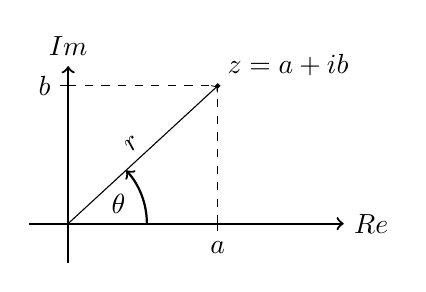
\begin{tikzpicture}
        \draw[->,thick] (-0.5,0)--(3.5,0) node[right]{$\operatorname{Re}$};
        \draw[->,thick] (0,-0.5)--(0,2) node[above]{$\operatorname{Im}$};
        \draw (1.9,0.1)--(1.9,-0.1) node[below]{$a$};
        \draw (0.1,1.75)--(-0.1,1.75) node[left]{$b$};
        \draw[dashed] (1.9,0)--(1.9,1.75); 
        \draw[dashed] (0,1.75)--(1.9,1.75);
        \draw[fill] (1.9,1.75) circle[radius=0.025] node[above right]{$z=a+ib$};
        \draw[->] (0,0)--(1.9,1.75) node[midway,sloped,above]{$r$};
        \draw[->,thick] (1,0) arc[radius=1,start angle = 0, end angle = 42.5];
        \draw[fill] (0.85,0) circle[radius=0] node[above left]{$\theta$};
    \end{tikzpicture}
\end{minipage}
\begin{align*} 
    z &= r(\cos\theta + i\sin\theta)\qquad r,r' \in \mathbb{R}_+ \cup \{0\} \\
    z &= r(\cos\theta' + \sin\theta') \\
    zz' &= (rr')((\cos\theta\cos\theta' - \sin\theta\sin\theta') + 
    i(\cos\theta\sin\theta' + \cos\theta'\sin\theta)) = \\ 
        &= (rr')(\cos(\theta+\theta') + i\sin(\theta+\theta'))
\end{align*}
\begin{df} 
    Jeśli $z = r(\cos\theta + i\sin\theta)$, gdzie $r \in \mathbb{R}_+ \cup \{0\}$, to 
    \begin{align*}
        r & \overset{\text{ozn}}{=} |z| \text{ nazywamy modułem } z.\\
        \theta & \overset{\text{ozn}}{=} \arg z \text{ nazywamy argumentem } z
    \end{align*}
    \footnotetext{$arg: \mathbb{C} \setminus \{0\} \to (\mathbb{R} , +_{\operatorname{mod} 2\pi})$}
\end{df}
\begin{ft} 
    \begin{align*}
        |z \cdot w| &= |z| \cdot |w| \\ 
        \arg(z \cdot w) &= \arg z + \arg w \quad (\operatorname{mod} \ 2\pi) 
    \end{align*}
\end{ft}
\begin{ft} 
    \begin{align*}
        |a + ib| &= \sqrt{a^2 + b^2} \\
        \arg (a+ib) &= \begin{cases} 
                        \operatorname{arctg} \frac{b}{a} & a \neq 0 \\
                        (\operatorname{sgn} b)\frac{\pi}{2} & a = 0
                    \end{cases}
    \end{align*} 
\end{ft} 
\begin{wn} (wzór de Moivre'a) 
    \[ (\cos\theta + i\sin\theta)^n = \cos(n\theta) + i\sin(n\theta) \]  
\end{wn}
\begin{dd} 
    dla $n \in \mathbb{Z}_+$ prosta indukcja,
    dla $n \in \mathbb{Z}_-$ ćwiczenia 
\end{dd} 
\begin{wn}
    \begin{align*}
        z &= r(\cos\theta + i\sin\theta) \\
        z^n &= r^n(\cos(n\theta)+i\sin(n\theta))
    \end{align*}
\end{wn} 
\begin{prz}
    $(1+i)^{100} = -2^{50}$
\end{prz}

\begin{df} 
    \[ e^{x+iy} = e^x(\cos y + i\sin y) \quad \text{ dla } x,y \in \mathbb{R} \] 
    $ \exp: \mathbb{R} \to \mathbb{R} $ \\ 
    $\exp : \mathbb{C} \to \mathbb{C} $
\end{df}
\begin{ft} 
    \[ e^z \cdot e^w = e^{z+w} \quad \text{dla }z,w \in \mathbb{C} \]
\end{ft}
\begin{dd} 
    \begin{align*}
         e^z \cdot e^w &= e^{x +iy} \cdot e^{a + ib} = e^x(\cos y + i \sin y) + e^a(\cos b + i\sin b) \\ 
    &= e^{x+a}(\cos(y+b) + i\sin(y+b)) = e^{(x+a) + i(y+b)} = e^{z+w}  
    \end{align*}
    \hfill \qed
\end{dd} 
\begin{wn} (wzór Eulera) \[ e^{i\pi} + 1 = 0 \] \end{wn}
\subsection{Pierwiastkowanie liczb zespolonych}
$\sqrt{-1} = ?$ \\ 
Chcemy znaleźć funkcję taką, że: 
\begin{align*}
    \sqrt{} &: \mathbb{C} \to \mathbb{C}  \\ 
        &(\sqrt{z})^2 = z  \\ 
        & \text{ciągła} 
\end{align*}
Taka funkcja nie istnieje 
\begin{align*}
    &z = r(\cos\theta + i\sin\theta) \\
    &w^2 = z (\text{myślimy, że} w = \sqrt{z}) \\
    &w = p(cos\varphi + i\sin\varphi) \\
  &\begin{cases} 
        p^2 = r \to p = \sqrt{r} \text{ pierwiastek rzeczywisty} \\
        2*\varphi = \theta \operatorname{mod} 2\pi
    \end{cases}  \\
    &w_1 = \sqrt{r} (\cos\frac{\theta}{2} + i\sin\frac{\theta}{2}) \\ 
    &w_2= \sqrt{r}(\cos\frac{\theta + 2\pi}{2} + i\sin\frac{\theta+2\pi}{2}) \end{align*}
\begin{figure}[!ht]
\centering
    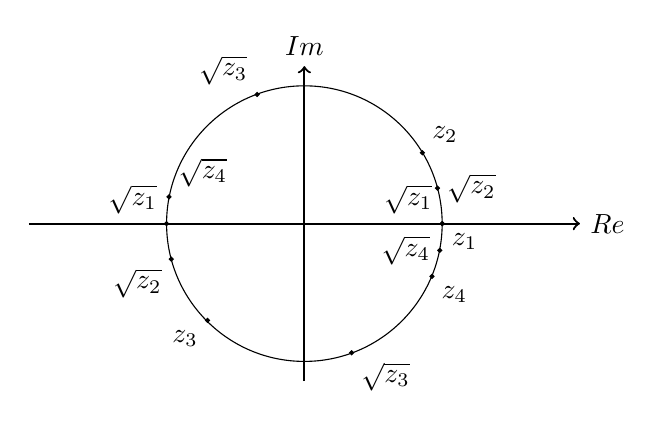
\begin{tikzpicture}
        \draw[->,thick] (-3.5,0)--(3.5,0) node[right]{$\operatorname{Re}$};
        \draw[->,thick] (0,-2)--(0,2) node[above]{$\operatorname{Im}$};
        \draw circle[radius=1.75];
        \draw[fill] (1.75,0) circle[radius=0.025] node[below right]{$z_1$};
        \draw[fill] (1.75,0) circle[radius=0.025] node[above left]{$\xcancel{\sqrt{z_1}}$};
        \draw[fill] (-1.75,0) circle[radius=0.025] node[above left]{$\sqrt{z_1}$};
        \draw[fill] (1.5,0.9) circle[radius=0.025] node[above right]{$z_2$};
        \draw[fill] (1.69,0.45) circle[radius=0.025] node[right]{$\xcancel{\sqrt{z_2}}$};
        \draw[fill] (-1.69,-0.45) circle[radius=0.025] node[below left]{$\sqrt{z_2}$};
        \draw[fill] (-1.23,-1.23) circle[radius=0.025] node[below left]{$z_3$};
        \draw[fill] (-0.6,1.64) circle[radius=0.025] node[above left]{$\xcancel{\sqrt{z_3}}$};
        \draw[fill] (0.6,-1.64) circle[radius=0.025] node[below right]{$\sqrt{z_3}$};
        \draw[fill] (1.62,-0.67) circle[radius=0.025] node[below right]{$z_4$};  
        \draw[fill] (-1.72,0.34) circle[radius=0.025] node[above right]{$\xcancel{\sqrt{z_4}}$}; 
        \draw[fill] (1.72,-0.34) circle[radius=0.025] node[left]{$\sqrt{z_4}$};
    \end{tikzpicture}
    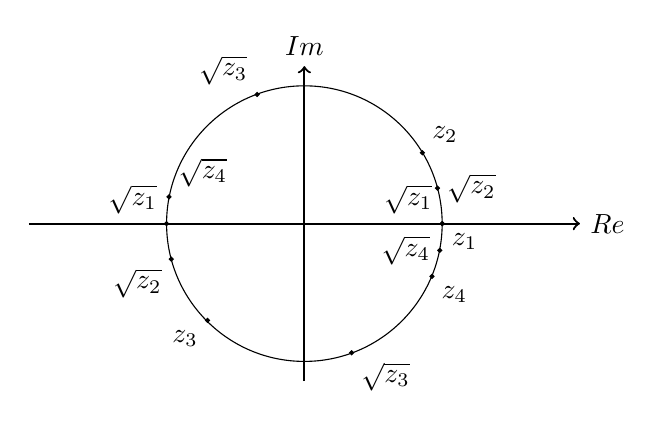
\begin{tikzpicture}
        \draw[->,thick] (-3.5,0)--(3.5,0) node[right]{$\operatorname{Re}$};
        \draw[->,thick] (0,-2)--(0,2) node[above]{$\operatorname{Im}$};
        \draw circle[radius=1.75];
        \draw[fill] (1.75,0) circle[radius=0.025] node[below right]{$z_1$};
        \draw[fill] (1.75,0) circle[radius=0.025] node[above left]{$\sqrt{z_1}$};
        \draw[fill] (-1.75,0) circle[radius=0.025] node[above left]{$\xcancel{\sqrt{z_1}}$};
        \draw[fill] (1.5,0.9) circle[radius=0.025] node[above right]{$z_2$};
        \draw[fill] (1.69,0.45) circle[radius=0.025] node[right]{$\sqrt{z_2}$};
        \draw[fill] (-1.69,-0.45) circle[radius=0.025] node[below left]{$\xcancel{\sqrt{z_2}}$};
        \draw[fill] (-1.23,-1.23) circle[radius=0.025] node[below left]{$z_3$};
        \draw[fill] (-0.6,1.64) circle[radius=0.025] node[above left]{$\sqrt{z_3}$};
        \draw[fill] (0.6,-1.64) circle[radius=0.025] node[below right]{$\xcancel{\sqrt{z_3}}$};
        \draw[fill] (1.62,-0.67) circle[radius=0.025] node[below right]{$z_4$};  
        \draw[fill] (-1.72,0.34) circle[radius=0.025] node[above right]{$\sqrt{z_4}$}; 
        \draw[fill] (1.72,-0.34) circle[radius=0.025] node[left]{$\xcancel{\sqrt{z_4}}$};
    \end{tikzpicture}
    \caption{widać, że pierwiastek nie może być ciągły}
\end{figure}
$\sqrt{}$ na $\mathbb{C}$ jest funkcją wielowartościową.
\begin{ft} 
    Jeśli $ z = r(\cos\theta + i\sin\theta), r \in\mathbb{R}_+$ to $w^n=z$ ma następujące $n$ pierwiastków: 
    \[ w_k = \sqrt[n]{r} (\cos\frac{\theta+2k\pi}{n}+i\sin\frac{\theta+2k\pi}{n}) \quad 
    \text{, dla }k = 0,1,\ldots,n-1 \]
\end{ft}
\begin{prz} $\sqrt{-1} = \pm i$ \end{prz} 
\begin{prz} 
    $\sqrt{i} = ?$ 
    \begin{align*}
        i = (\cos\frac{\pi}{2} &+ i\sin\frac{\pi}{2}) \\
        w_1 = (\cos\frac{5\pi}{4} + i\sin\frac{5\pi}{4})=-\frac{1+i}{2} & \qquad  w_2 = (\cos\frac{\pi}{4} + i\sin\frac{\pi}{4}) = \frac{1+i}{2} 
    \end{align*}
\end{prz}
\begin{uw} $\sqrt[n]{0} = 0 $ \end{uw}
\begin{tw} (zasadnicze twierdzenie algebry) \\ 
    Każdy wielomian zespolony ($P \in \mathbb{C}[x]$) (niestały) ma pierwiastek. 
    \footnotetext{$\mathbb{C}$ jest ciałem algebraicznie domkniętym}
\end{tw} 
\begin{dd}
    Formalny dowód $\rightarrow$ topologia algebraiczna (pojęcie grupy podstawowej). \\ 
    Idea dowodu (nie wprost): \\ 
    $P \in \mathbb{C}[z],\ P(z) = a_n z^n + \ldots + a_1 z + a_0, \ a_in \in \mathbb{C}, a_n \neq 0$
    Zakładamy nie wprost, że $P$ nie ma pierwiastków. 
    $P: \mathbb{C} \xrightarrow{\text{ciągłe}} \mathbb{C} \setminus \{0\} \xrightarrow{\text{ciągłe}} 
    S^1 = \{z \in \mathbb{C} : |z| = 1\}$ \\ 
    $z \mapsto \frac{P(z)}{|P(z)|}$ \\ 
    $F: \overscript{\mathbb{C}}{\cap}{S^1} \to S^1 \quad F(z) = \frac{P(z)}{|P(z)|}$ \\ 
    $fr: \underscript{S^1}{\vertni}{z} \to \underscript{S^1}{\vertni}{\frac{P(z)}{|P(z)|}} \quad
    r \in \mathbb{R}_+,\ |z| = r$ \\
    %rysunek z dużą ilością kułek xD 
    $n(r) \in \mathbb{Z}$ - znakowana liczba nawinięć sznurka na szpulkę nici. (jest niezmienna, 
    dowód właśnie z topologii algebraicznej). \\ 
    $n : \mathbb{R}_+ \mapsto \mathbb{Z}$ jest ono ciągłe, czyli jest stałe! \\ 
    $r: \ P(z) \simeq a \ \to \ n(r) = 0$ \\ 
    $R: \ P(z) \simeq a_n z^n \to n(R) = \deg P$ \hfill \lightning
\end{dd} 
\begin{wn} 
    Jeśli $P \in \mathbb{C}[x]$, to $P$ ma \underline{dokładnie} $\operatorname{deg} P$ pierwiastków 
    (licząc z krotnościami).
\end{wn}
\begin{wn} 
    Każdy wielomian zespolony (niestały) rozkłada się na iloczyn wielomianów liniowcyh \end{wn} 
\begin{dd} 
    $P(z) $ma pierwiastek a.\\ 
    $P(z) = (z-a)Q(z) \quad$ (tw. Bezout'a), a dalej indukcja \hfill \qed
\end{dd} 
\begin{ft} 
    Jesli $P \in \mathbb{R}[x], \ z \in \mathbb{C} $ oraz $P(z) = 0$, to $P(\overline{z}) = 0$. \\ 
    Co więcej krotność $z$ = krotność $\overline{z}$.
\end{ft}
\begin{dd} 
    \begin{align*} 
        &P(x) = a_nx^n + \ldots + a_1x + a_0 \\ 
        0 &= P(z) = a_nz^n + \ldots + a_1z + a_0 \\ 
        \overline{0} &= \overline{a_nz^n + \ldots + a_1z+a_0}\\ 
        0 &= \overline{a_nz^n} + \ldots + \overline{a_1z} + \overline{a_0} \\ 
        0 &= a_n(\overline{z})^n + \ldots + a_1\overline{z} + a_0 = P(\overline{z}) \\
    \end{align*} 
\end{dd} 
\begin{wn} 
    Każdy wielomian rzeczywisty $(P \in \mathbb{R}[x])$ rozkłada się na iloczyn czynników liniowych i kwadratowych
\end{wn}
\begin{dd} 
    \begin{align*} 
        P(x) & = (x-z)(x-\overline{z})Q(x) \quad Q \in \mathbb{C}[x] \\  
        \underscript{P(x)}{\vertin}{\mathbb{R}[x]} & = \underscript{(x^2 - 2ax + (a^2 + b^2))}{\vertin}{\mathbb{R}[x]}Q(x) \\ 
        \text{czyli } Q &\in \mathbb{R}[x] \text{ i kontynuacja indukcyjnie}
    \end{align*}
\end{dd} 
\begin{prz} Zadanie 31 z listy 7 
    \[ \begin{pmatrix} 2\sqrt{3} & -7 \\ 1 & -\sqrt{3} \end{pmatrix}^{100} \cdot \begin{pmatrix} 1 \\ 2 \end{pmatrix} \]
    \begin{align*}    
        \det \begin{pmatrix} 2\sqrt{3} & -7 \\ 1 & -\sqrt{3} \end{pmatrix} = (x-2\sqrt{3})(x+\sqrt{3}) + 7 = \\ 
        = x^2 - \sqrt{3}x + 1 \\ 
        \Delta = 3 - 4 = -1 \\ 
        \sqrt{\Delta} = \pm i \\ 
        x = \frac{\sqrt{3} \pm i}{2} \\ 
    \end{align*}
    \begin{align*}
        &\begin{pmatrix} 2\sqrt{3} & -7 \\ 1 & -\sqrt{3} \end{pmatrix} \cdot \begin{pmatrix} a \\ b \end{pmatrix} = 
        \frac{\sqrt{3} + i}{2} \begin{pmatrix} a \\ b \end{pmatrix} \\
        \begin{cases} 
            2\sqrt{3}a - 7b = \frac{\sqrt{3}+i}{2}a \\
            a - \sqrt{3} b = \frac{\sqrt{3}+i}{2} b
        \end{cases} \\ 
        &\begin{cases} 
            \cancel{\frac{3\sqrt{3}-i}{2} a - 7b = 0}\footnotemark \\ 
            a - \frac{3\sqrt{3}+i}{2}b = 0
        \end{cases} \\ 
        & a = \frac{3\sqrt{3} + i}{2} b \\ 
        \lambda_1 = \frac{\sqrt{3}+i}{2} & \qquad v_1 = \begin{pmatrix} 3\sqrt{3}+i \\ 2 \end{pmatrix} \\ 
        \lambda_2 = \frac{\sqrt{3}-i}{2} & \qquad v_2 = \begin{pmatrix} 3\sqrt 3-i \\ 2 \end{pmatrix} 
    \end{align*}
\end{prz}
\footnotetext{A tam liniowo zalezne krab}
\begin{ft} 
    Jeśli $A \in M_{n\times n}(\mathbb{R})$, zaś $\lambda \in \mathbb{C} \setminus \mathbb{R}$ jest 
    wartością własna $A$, a jej wektor własny to $v \in \mathbb{C}^n$, to $\overline{v} \in \mathbb{C}^n$ jest
    wektorym własnym $A$ dla wartości $\overline{\lambda}$.
\end{ft} 
\begin{dd} 
    $\chi_A \in \mathbb{R}[x]$, więc $\chi_A (\lambda ) = 0 \Rightarrow \chi_A(\overline{\lambda}) = 0$ \\ 
    $Av = \lambda v$ \\ 
    $\overline{Av} = \overline{\lambda v}$ \\ 
    $\overline{A} \cdot \overline{v} = \overline{\lambda} \cdot \overline{v} $ \\ 
    $ A \cdot \overline{z} = \overline{\lambda} \cdot \overline{z}$ \\ 
    czyli $\overline{v}$ to wektory własny dla $\overline{\lambda}$. \hfill \qed
\end{dd} 
\begin{prz} Zadanie 31 lista 7, ale inaczej
    \begin{align*}
        A &= P \begin{pmatrix} \lambda_1 & 0 \\ 0 & \lambda_2 \end{pmatrix} P^{-1} \\
        A^n &= P \begin{pmatrix} \lambda_1^n & 0 \\ 0 & \lambda_2^n \end{pmatrix} P^{-1} = 
        \begin{pmatrix} a_{11} & a_{12} \\ a_{21} & a_{22} \end{pmatrix} \\ 
        a_{ij} &= \alpha_{ij} \lambda_1^n + \beta_{ij} \lambda_2^n \text{, gdzie } \alpha_{ij},\beta_{ij} 
        \text{ nie zależą od } n. \\
        \lambda_1 &= \frac{\sqrt{3}+i}{2}, \quad \lambda_2 = \frac{\sqrt{3}-i}{2} \\ 
        &\begin{cases}
            a_n = \alpha (\frac{\sqrt{3}+i}{2})^n + \alpha' (\frac{\sqrt{3}-i}{2})^n \\ 
            b_n = \beta (\frac{\sqrt{3}+i}{2})^n + \beta' (\frac{\sqrt{3}-i}{2})^n 
        \end{cases} \\
        &\underline{n=0} \\ 
        &\begin{cases}
            1 = a_0 = \alpha + \alpha' \\ 
            2 = b+0 = \beta + \beta' 
        \end{cases} \\ 
        &\underline{n=1} \\ 
        &\begin{cases}
            2\sqrt{3} - 14 = a_2 = \alpha (\frac{\sqrt{3}+i}{2}) + \alpha' (\frac{\sqrt{3}-i}{2}) \\ 
            1 - 2\sqrt{3} = b_2 = \beta (\frac{\sqrt{3}+i}{2}) + \beta' (\frac{\sqrt{3}-i}{2})
        \end{cases} \\ 
        &\text{Z tego da się obliczyć } \alpha,\alpha',\beta,\beta'
    \end{align*}
\end{prz} 
\begin{uw} $a_{ij} = \alpha_{ij} \lambda_1 ^n + \beta_{ij} \lambda^n_2$ opisuje nam jak $a_{ij}$ będzie się 
    zachowywać ( o tym który z czynników $\lambda_1,\lambda_2$ dominuje decyduje ich moduł) 
    (opisuje asymptotykę). \end{uw}
\begin{uw} Pytanie z publiczności (jakby ktoś chciał je poznać to proszę do Mateusza Rzepeckiego).\\
    $\lambda = r(\cos\theta + i\sin\theta)$ \\ 
    $\overline\lambda = r(\cos\theta-i\sin\theta)$ \\ 
    $ \alpha = s(\cos\varphi + i\sin\varphi)$ \\ 
    $a_n = \alpha (\lambda)^n + \beta (\overline\lambda)^n \in \mathbb{R}$ dla dowolnego n \\
    $\overline\beta \lambda^n + \beta(\overline\lambda)^n \in \mathbb{R}$, odejmując otrzymujemy: \\ 
    $(\alpha - \overline\beta) \lambda^n \in \mathbb{R}$ dla dowolnego n, czyli $\alpha = \overline\beta$\\ 
    $a_n = \alpha \lambda^n + \overline\alpha (\overline\lambda)^n = 2 \operatorname{Re}(\alpha\lambda^n)$ \\ 
    $a_n = 2sr^n \cos(\varphi + n\theta)$
\end{uw} 
\section{Suma prosta} 
\begin{minipage}[c]{0.5\textwidth}
$V$ \\ 
baza $B = (b1,\ldots,b_n)$ \\ 
$F: V \to V$ \\ 
$W = \operatorname{Lin} \{ b_1,\ldots,b_k\} < V$ \\ 
$W' = \operatorname{Lin}\{ b_{k+1},\ldots,b_n\} < V$ 
\end{minipage}%
\begin{minipage}[c]{0.4\textwidth}
\begin{tikzpicture}
    \matrix[matrix of nodes,nodes in empty cells, left delimiter = (, right delimiter = )] (m)
    { 
         &  &  & & & &\\
         &  &  & & 0& &\\
         &  &  & & & &\\
         &  &  & & & &\\ 
         &  0&  & & & &\\
         &  &  & & & &\\
    };
    \draw (m-1-1.north) -- (m-3-1.south) node[midway, left]{$n$}; 
    \draw (m-1-1.north) -- (m-1-3.north) node[midway, above]{$n$};
    \draw (m-3-1.south) -- (m-3-3.south);
    \draw (m-3-3.south) -- (m-1-3.north);

    \draw (m-3-3.south east) -- (m-3-6.south east);
    \draw (m-3-6.south east) -- (m-6-6.south east) node[midway,above,sloped]{$n-k$};
    \draw (m-6-6.south east) -- (m-6-3.south east) node[midway,below]{$n-k$};
    \draw (m-6-3.south east) -- (m-3-3.south east);
\end{tikzpicture}
\end{minipage} \\
Niech $W,W' - F -$ niezmiennicze. \\
$F: V \to V \rightsquigarrow F_{|_W}: W \to W, \ F_{|_{W'}}: W' \to W'$ \\
$V = W \oplus W'$ (suma prosta podprzestrzeni $W$ i $W'$).
\begin{df} 
    Przestrzeń liniowa $V$ jest \underline{sumą prostą} przestrzeni $V_1,\ldots,V_n < V$ \\ 
    (ozn. $V = V_1 \oplus \ldots \oplus V_n = \underset{i=1}{\overset{n}{\oplus}} V_i$), jeśli 
    każdy wektor $v \in V$ przedstawia się \underline{jednoznacznie} w postaci $v = v_1+\ldots+v_n$, gdzie 
    $v_i \in V_i$.
\end{df} 
\begin{prz} 
    $B = (b_1,\ldots,b_n)$ - baza $V$ \\ 
    $V = \operatorname{Lin}\{b_1\} \oplus \ldots \oplus \operatorname{Lin}\{b_n\}$
\end{prz}
\begin{prz} 
    $B = (b_1,\ldots,b_n)$ - baza $V$ \\ 
    $V = \operatorname{Lin}\{b_1,\ldots,b_k\} \oplus \operatorname{Lin}\{b_{k+1},\ldots,b_n\}$ \\ 
    $V \ni v = (\alpha_1 b_1 + \ldots + \alpha_k b_k) + (\alpha_{k+1} b_{k+1} + \ldots + \alpha_n b_n)$ 
\end{prz} 
\begin{prz} 
    \begin{align*}
        \mathbb{R}[x] = \{ P \in \mathbb{R}[x] : P(-x) &= P(x) \} = \operatorname{Lin}\{1,x^2,x^4,\ldots\} \\ 
        &\oplus \\ 
        \{ P \in \mathbb{R}[x] : P(-x) &= -P(x) \}  \\ 
    \end{align*}
    \[P(x) = \frac{P(x)+P(-x)}{2} + \frac{P(x) - P(-x)}{2} \]
\end{prz}
\begin{prz} 
    $\mathbb{R}^3 = \left\{ \begin{pmatrix} x \\ y \\ z \end{pmatrix}: x + y + z = 0 \right\} \oplus 
    \left\{ t \begin{pmatrix} 1 \\ 1 \\ 1 \end{pmatrix}, t \in \mathbb{R} \right\} $
\end{prz}
\begin{df} 
    Podprzestrzenie $V_1,\ldots,V_n < V$ nazywamy lnz jeśli: 
    \[ (\forall v_1 \in V_1,\ldots,v_n \in V_n) \quad v_1 + \ldots +v_n = 0 \Rightarrow v_1 = \ldots = v_n = 0 \]
\end{df} 
\begin{prz} 
    $V_i = \operatorname\{v_i\}$ \\ 
    $V_1,\ldots,V_n$ lnz $\Leftrightarrow v_1,\ldots,v_n$ lnz 
\end{prz}
\begin{lem}
    $V_1,\ldots,V_n < V$ lnz $\Leftrightarrow \forall i (V_i \cap (V_1+\ldots+\widehat{V_i} + \ldots + V_n) = \{0\})$
    \begin{dd} \hfill 
        \begin{itemize} 
            \item[$\Rightarrow$] $v_i \in V_i \setminus \{0\}$, gdyby \\ 
                $v_i = v+1 + \ldots + \widehat{v_i} + \ldots + v_n$ \\ 
                $v_1 + \ldots - v_i + \ldots + v_n = 0$ \hfill \lightning
            \item[$\Leftarrow$] wprost \\ 
                $v_1 + \ldots + v_n = 0$ \\ 
                $v_i = -v_1 - v_2 - \ldots - \widehat{v_i} - \ldots - v_n$ \\ 
                $V_i \cap (V_1 + \ldots + \widehat{V_i}+ \ldots + V_n) = \{0\}$ \\ 
                czyli $v_i = 0 $ dla dowolnego $i$. \hfill \qed
        \end{itemize}
    \end{dd} 
\end{lem}
\begin{wn} 
    $V_1,V_2 < V$ lnz $\Leftrightarrow V_1 \cap V_2 = \{0\}$
\end{wn} 
\begin{df}[nobreak = true]
    Jeśli $V_1,\ldots,V_n$ to dowolne przestrzenie liniowe nad $K$, to \underline{produktem} $V_1,\ldots,V_n$ 
    nazywamy zbiór: 
        \[ V_1 \times V_2 \times \ldots \times V_n \text{, z działaniami }\] 
     \begin{align*} 
        (v_1,\ldots,v_n)+(v_1',\ldots,v_n') &= (v_1 + v_1',\ldots,v_n+v_n') \\ 
        \alpha (v_1,\ldots,v_n) &= (\alpha v_1,\ldots,\alpha v_n)
    \end{align*}
\end{df} 
\begin{ft} 
    $V_1,\ldots,V_n$ jest przestrzenią liniową
\end{ft} 
\begin{dd} 
    ćw 
\end{dd} 
\begin{przy} \hfill 
    \begin{itemize} 
        \item $\mathbb R^2 = \mathbb R \times \mathbb R$
        \item $K^n = \underbrace{K \times K \times \ldots \times K}_{n}$
    \end{itemize} 
\end{przy} 
\begin{ft} 
    Niech $V_1,\ldots,V_n < V$. Wówczas NWSR:
    \begin{enumerate}[(1)]
        \item $V = V_1 \oplus \ldots \oplus V_n$
        \item $V_1,\ldots,V_n$ lnz oraz $V_1+\ldots,V_n=V$
        \item $\phi : V_1 \times V_2 \times \ldots \times V_n \to V$ jest izomorfizem \\
        Jeśli $\dim V < \infty$
        \item $V_1,\ldots,V_n$ lnz oraz $\dim V_1 + \ldots + \dim V_n = \dim V$ 
        \item $V_1+\ldots + V_n = V$ oraz $\dim V_1 + \ldots + \dim V_n = \dim V$
    \end{enumerate}
\end{ft} 
\begin{lem} \label{indeksior}
    $\dim (V_1 \times \ldots \times V_n) = \dim V_1 + \ldots + \dim V_n$
    \begin{dd} 
        $(0,\ldots,0,b_{i,i_k},0,\ldots,0),\ 1 \le i_k \le \dim V_k$
        jest bazą. $V_1 \times \ldots \times V_n$. Reszta zostawione jako ćwiczenie.
        \footnotetext{$b_{k,1},\ldots,b_{k,\dim V_k}$ jest bazą $V_k$}
    \end{dd} 
\end{lem} 
\begin{dd}  \hfill
    \begin{itemize} 
        \item[$(1) \Rightarrow (2)$] $V_1,\ldots,V_n$ lnz: \\ 
            $v_1 + \ldots + v_n = 0$. Z jednoznaczności $v_i = 0$. \\ 
            $V_1 + \ldots + V_n = V$: \\ 
            $V \ni v = v_1 + \ldots v+n$ z def.
        \item [$(2) \Rightarrow (3)$] $\phi$ jest liniowe. \\ 
            $\phi$ jest "na", bo $V_1+\ldots+V_n = \operatorname{Im} \phi = V$ \\ 
            $\phi$ jest różnowartściowe, bo $\ker \phi = \{ (v_1,\ldots,v_n): v_1+\ldots+v_n = 0\} = 
            \{(0,\ldots,0)\}$, bo $(V_1,\ldots,V_n)$ są lnz. 
        \item [$(3) \Rightarrow (1)$] $v \in V$ \\ 
            $v_i \in V_i$, takie, że $v = (v_1 + \ldots + v_n)$ \\ 
            $v = \phi (v_1,\ldots,v_n)$ \\ 
            $\phi$ jest izomorfizmem ,więc $\exists ! (v_1,\ldots,v_n)$ 
        \item [$(3) \Leftrightarrow (4)$] 
        \item [$(3) \Leftrightarrow (5)$] tw. o indeksie dla $\phi$: \\ 
            $\dim V_1 + \ldots \dim V_n = \dim \ker \phi + \dim \operatorname{Im} \phi = 
            \dim \ker \phi + \dim (V_1+\ldots+V_n)$
            \begin{align*} 
                \dim V_1 + \ldots V_n &= \dim (V_1 + \ldots + V_n) \\ 
                &\Updownarrow  \\ 
                \ker \phi &= \{ 0\} \\ 
                \dim (V_1 + \ldots + V_n) &= \dim V \\ 
                &\Updownarrow \\ 
                V &= V_1 + \ldots V_n \\
                \phi \text{ jest} &\text{ izomorfizmem} \\ 
                 &\Updownarrow \\ 
                \ker \phi = \{ 0\} &\text{ oraz } \operatorname{Im} \phi = V
            \end{align*}  
    \end{itemize} 
\end{dd} 
\begin{wn} 
    Jeśli $V_1,V_2 < V, \ \dim V < \infty$ to NWSR:
    \begin{enumerate}[(1)]
        \item $V = V_1 \oplus V_2$
        \item $V_1 \cap V_2 = \{ 0\}$ oraz $V_1 + V_2 = V$
        \item $V_1 \cap V_2 = \{ 0\}$ oraz $\dim V_1 + \dim V_2 = \dim V$ 
        \item $V_1 + V_2 = V$ oraz $\dim V_1 + \dim V_2 = \dim V$
    \end{enumerate} 
\end{wn}
\begin{lem} 
    Dla dowolnej $W < V$ istnieje $W' < V$ (tw. o podprzestrzeni dopełniczej) taka, że \[V = W \oplus W'\]
    \begin{dd} Był na cwiczeniach \end{dd} 
\end{lem} 
\begin{df} 
    Niech $F: V \to V,\ W < V \ W$ jest $F-$ niezmiennicza, jesli \[ (\forall w \in W) (F(w) \in W)\]
\end{df}
\begin{ft} 
    $F: V \to V,\ \lambda_1,\ldots,\lambda_n$ - parami różne wartości własne, to $V_{\lambda_1},\ldots,
    V_{\lambda_n}$ są lnz oraz są $F-$ niezmiennicze.
\end{ft} 
\begin{wn} 
    $V = V_{\lambda_1} \oplus \ldots \oplus V_{\lambda_n} \oplus W$ dla pewnej $W < V$
\end{wn} 
\begin{ft} 
    $F: V \to V$ liniowe \\ 
    $V_1,\ldots,V_n$ - $F-$ niezmiennicze \\ 
    $V = V_1 \oplus \ldots \oplus V_n$ 
    Wówczas $\chi_F = \chi_{F|{V_1}} \cdot \ldots \cdot \chi_{F|V_n}$
\end{ft} 
\begin{dd} ~\\ 
    $B_i$ - baza $V_i$ \\ 
    $B = \cdot \hspace{-7.5pt}\bigcup B_i$ - baza $V$ %xDDDDDDDDDDDDDDDDDDDDDDDDDDDDDDDDDDDDDDd
    \[ m_B^B (F) = 
        \begin{pmatrix} 
            m_{B_1}^{B_1} (F_{|V_1}) & & &  \\ 
                                     &  m_{B_2}^{B_2} (F_{|V_2}) & & \\ 
                                     & & \ddots & \\ 
                                     & & &   m_{B_n}^{B_n} (F_{|V_n}) 
        \end{pmatrix} 
    \]
    \[ \det (m_B^B (F) - xI) = \prod_{i=1}^n \det (m_{B_i}^{B_i} (F_{|V_i}) -xI)\]
\end{dd} 
\begin{ft} 
    Jeśli $F: V \to V$ liniowy, $W$ jest $F-$ niezmienniczą podprzestrzenią $V$ oraz $\overline F: V/_{W} \to V/_W$ \\ 
    zdefiniowane $\overline F (v+W) = F(v) + W$, to $\chi_F = \chi_{F|_w} \cdot \chi_{\overline F}$
\end{ft} 
\begin{dd} ~\\ 
    $\overline F$ dobrze zdefiniowane 
    \begin{align*}
        v+1 + W &= v_2 + W  \\ 
                &\Updownarrow \\
        v_1 - v_2 &\in W  \\ 
                  &\Downarrow  \\ 
        F(v_1) - F(v_2) &\in W \\ 
                        &\Updownarrow \\
        F(v_1) + W &= F(v_2) + W
    \end{align*} 
    $v_1 - v_2 \in W \Rightarrow F(v_1 - v_2) \in W$ \\ 
    $\overline F$ liniowe (ćw) \\ 
    $\mathcal B = (b_1,\ldots,b_k)$ - baza W \\ 
    $\mathcal B' = (b_1,\ldots,b_k,b_{k+1},\ldots,b_n)$ - baza V \\ 
    baza $V/_W = \overline B (b_{k+1}+W,\ldots,b_n+W)$ \\ 
    $m_{B'}^{B'} (F) = \begin{pmatrix} m_B^B (F_{|W}) & \ast \\ 0 & m_{\overline B}^{\overline B}(\overline F) \end{pmatrix}$ \\
    $\det(m_{B'}^{B'} (F) - xI) = \det (m_B^B (F_{|{W}}) - Ix) \cdot 
    \det (m_{\overline B}^{\overline B} (\overline F) - xI)$
\end{dd}
\section{Diagonalizacja macierzy} 
\begin{enumerate} 
    \item Wartość, wektory własne $\to$ diagonalizować 
    \item Przeszkoda 1: $\chi_F$ ma za mało pierwiastków \\ 
        Rozwiązanie: $\mathbb C$ zamiast $\mathbb R$
    \item Przeszkoda 2: za małe przestrzenie własne ($\dim V_\lambda < $ krotność $\lambda$)\\
        Rozwiązanie (częściowe): \underline{tw. Jordana}: \\
        Każda macierz można zapisać w postaci 
        \[ PJP^{-1}, \ \text{gdzie } J = \begin{pmatrix} J_1 & & \\ & \ddots & \\ & & J_k \end{pmatrix}
        \text{, a } J_i = \begin{pmatrix} \lambda_i & 1 & & & \\ & \ddots & \ddots & & \\ 
            & & \ddots & 1 \\ & & &  \lambda_i \end{pmatrix}
        \]
    \item Ulubione macierze: macierze symetryczne. \\
        \underline{Tw. spektralne}: Macierz symetryczna nad $\mathbb R$ zawsze się diagonalizuje
        (i to nad $\mathbb R$) i do tego można wybrać bazę wektorów własnych złożoną z wektorów 
        parami prodopadłych.
    \item Co z macierzami prostokątnymi? subsytut diagonalizowalności dla macierzy prostokątnych $=$ rozkład SVD
\end{enumerate} 
\subsection{Po co diagonalizować}
\begin{enumerate} 
    \item Podnosić macierze do wysokich potęg. (np. macierz $A$ reprezentuje pewien proces który iterujemy 
        $n-$ krotnie.)
    \item $ A = P \begin{pmatrix} \lambda_1 & & \\ & \ddots & \\ & & \lambda_n \end{pmatrix} P^{-1} 
        \approx P \begin{pmatrix} \lambda_1 & & & & & \\ 
                                    & \ddots & & & & \\ 
                                    & & \lambda_k & & & \\ 
                                    & & & 0 & & \\ 
                                    & & & & \ddots & \\ 
                                    & & & & & 0 \end{pmatrix} P^{-1}$.\\ 
                                    Kompresja danych, jezeli $\lambda_1 > 
                                    \lambda_2 > \ldots > \lambda_n$, to można zgubić mniejsze.
\end{enumerate} 
\subsection{Rozwiązywanie rekurencji} 
$\begin{cases} 
    a_{n+1} = 5a_n - 6a_{n-1} \\ 
    a_1 = 2 \\ 
    a_0 = 3
\end{cases}$ \\ 
$\begin{pmatrix} 
    a_{n+1} \\ a_n
    \end{pmatrix} = \begin{pmatrix} 5 & -6 \\ 1 & 0 \end{pmatrix} \cdot \begin{pmatrix} a_n \\ a_{n-1}
    \end{pmatrix}$ \\ 
$\begin{pmatrix} a_1 \\ a_0 \end{pmatrix} \mapsto \begin{pmatrix} a_2 \\ a_1 \end{pmatrix} 
\mapsto \begin{pmatrix} a_3 \\ a_2 \end{pmatrix} \mapsto \ldots$  \\ 
$\begin{pmatrix} 
    a_{n+1} \\ a_n
    \end{pmatrix} = \begin{pmatrix} 5 & -6 \\ 1 & 0 \end{pmatrix}^n \cdot \begin{pmatrix} a_1 \\ a_0
    \end{pmatrix}$ \\
$\lambda_1 = 2 \quad v_1 = \begin{pmatrix} 2 \\ 1 \end{pmatrix}$ \\ 
$\lambda_2 = 3 \quad v_2 = \begin{pmatrix} 3 \\ 1 \end{pmatrix}$ \\ 
$\begin{pmatrix} 
    a_{n+1} \\ a_n
    \end{pmatrix} = \begin{pmatrix} 2 & 3 \\ 1 & 1 \end{pmatrix} 
    \cdot \begin{pmatrix} 2^n &  \\  & 3^n \end{pmatrix} 
    \cdot \begin{pmatrix} 2 & 3 \\ 1 & 1 \end{pmatrix}^{-1}
    \cdot \begin{pmatrix} 2 \\ 3 \end{pmatrix}$ \\
Dla dowolnych warunków początkowych mamy: \\
$\begin{pmatrix} 
    a_{n+1} \\ a_n
    \end{pmatrix} = \begin{pmatrix} 2 & 3 \\ 1 & 1 \end{pmatrix} 
    \cdot \begin{pmatrix} 2^n &  \\  & 3^n \end{pmatrix} 
    \cdot \begin{pmatrix} 2 & 3 \\ 1 & 1 \end{pmatrix}^{-1}
    \cdot \begin{pmatrix} \alpha \\ \beta \end{pmatrix}$ \\
\noindent\rule{\textwidth}{0.4pt}\\ 
$b_{n+1} = 4 b_n - 4 b_{n-1}$ \\
$\begin{pmatrix} 
    b_{n+1} \\ b_n
    \end{pmatrix} = \begin{pmatrix} 4 & -4 \\ 1 & 0 \end{pmatrix} \cdot \begin{pmatrix} b_n \\ b_{n-1}
    \end{pmatrix}$ \\ 
$\begin{pmatrix} 
    b_{n+1} \\ b_n
    \end{pmatrix} = \begin{pmatrix} 4 & -4 \\ 1 & 0 \end{pmatrix}^n \cdot \begin{pmatrix} b_1 \\ b_0
    \end{pmatrix}$ \\ 
$\lambda_1 = \lambda_2 = 2$\\ 
$ \dim V_2 = 1$ \\ 
$\begin{pmatrix} 4 & -4 \\ 1 & 0 \end{pmatrix} = P \begin{pmatrix} 2 & 1 \\ 0 & 2 \end{pmatrix} P^{-1}$ \\ 
$\begin{pmatrix} 4 & -4 \\ 1 & 0 \end{pmatrix}^n = P \begin{pmatrix} 2 & 1 \\ 0 & 2 \end{pmatrix}^n P^{-1}$ 
\begin{lem}
    $ \begin{pmatrix} \lambda & 1 \\ 0 & \lambda \end{pmatrix}^n = \begin{pmatrix} \lambda^n & n\lambda^{n-1} \\ 
    0 & \lambda^n \end{pmatrix}$ 
\begin{dd} 
    prosta indukcja na ćwiczenia
\end{dd} 
\end{lem} 
$\begin{pmatrix} 4 & -4 \\ 1 & 0 \end{pmatrix}^n = P \begin{pmatrix} 2^n & n2^{n-1} \\ 0 & 2^n 
\end{pmatrix} P^{-1}$ \\ 
$b_n = \begin{pmatrix} 0 & 1 \end{pmatrix} P \begin{pmatrix} 2^n & n2^{n-1} \\ 0 & 2^n \end{pmatrix} P^{-1} 
\begin{pmatrix} b_1 \\ b_0 \end{pmatrix}$ \\ 
$b_n = c_1 2^n + \frac{c_2}{2} n 2^n$
\subsection{Łańcuch Markowa (proces Markowa z czasem dyskretnym)}
(probabilistyczny automat skończony) \\ 
(błądzenie losowe po grafie skierowanym) \\
\textbf{Zadanie}:
Rzucamy $100$ razy monetą. Jakie jest prawdopodobieństwo, że wypadną (w którymkolwiek momencie) 3 orły pod rzad?\\
\begin{minipage}[c]{0.5\textwidth}
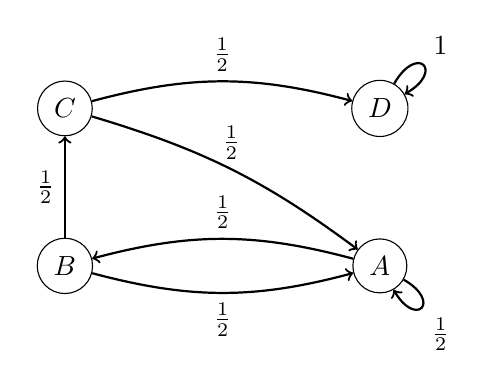
\begin{tikzpicture}
    \node[shape=circle,draw=black] (A) at (4,0) {$A$};
    \node[shape=circle,draw=black] (B) at (0,0) {$B$};
    \node[shape=circle,draw=black] (C) at (0,2) {$C$};
    \node[shape=circle,draw=black] (D) at (4,2) {$D$};
    \path[->,thick] (A) edge [out=330,in=300,looseness=8] node[below right]{$\frac{1}{2}$} (A);
    \path[->,thick] (A) edge [bend right = 15] node[above]{$\frac{1}{2}$} (B);
    \path[->,thick] (B) edge [bend right = 15] node[below]{$\frac{1}{2}$} (A);
    \path[->,thick] (B) edge node[left]{$\frac{1}{2}$} (C);
    \path[->,thick] (C) edge [bend left = 10] node[above]{$\frac{1}{2}$} (A);
    \path[->,thick] (C) edge [bend left = 15] node[above]{$\frac{1}{2}$} (D);
    \path[->,thick] (D) edge [out=60,in=30,looseness=8] node[above right]{$1$} (D);
\end{tikzpicture} 
\end{minipage}%
\begin{minipage}[c]{0.5\textwidth} 
    \centering
    \begin{tabular}{ |r| c| } 
        \hline
        ostatnie rzuty & sytuacja \\
        \hline 
        \ldots R & $A$ \\
        \ldots RO & $B$ \\
        \ldots ROO & $C$ \\ 
        \ldots OOO & $D$ \\
        \hline
    \end{tabular} 
\end{minipage}  \\ 
%-------------------------------------
Loop$a_n=$ prawdopodobieństwo znalezienie się w $A$ w $n$ krokach \\ 
$b_n=$ prawdopodobieństwo znalezienie się w $B$ w $n$ krokach \\ 
$c_n=$ prawdopodobieństwo znalezienie się w $C$ w $n$ krokach \\ 
$d_n=$ prawdopodobieństwo znalezienie się w $D$ w $n$ krokach  \\ 
$a_{n+1} = \frac{1}{2} a_n + \frac{1}{2} b_n + \frac{1}{2} c_n$ \\ 
$b_{n+1} = \frac{1}{2} a_n$ \\ 
$c_{n+1} = \frac{1}{2} b_n$ \\ 
$d_{n+1} = \frac{1}{2} c_n + d_n$ \\
$\begin{pmatrix} a_{n+1} \\ b_{n+1} \\ c_{n+1} \\ d_{n+1} \end{pmatrix} = 
\begin{pmatrix} \frac{1}{2} & \frac{1}{2} & \frac{1}{2} & 0 \\ 
                \frac{1}{2} & 0 & 0 & 0 \\ 
                0 & \frac{1}{2} & 0 & 0 \\ 
            0 & 0 & \frac{1}{2} & 1 \end{pmatrix} \cdot 
            \begin{pmatrix} a_n \\ b_n \\ c_n \\ d_n \end{pmatrix}$ \\ 
$X_{n+1} = M X_n$ \\ 
$M = (m_{ij})$ ma następujące właśności: 
\begin{enumerate} 
    \item $0 \le m_{ij} \le 1$ 
    \item $\sum\limits_{i=1}^n m_{ij} = 1$ (suma kolumy), dla wszystkich j
\end{enumerate} 
tzw. (lewa)\footnote{prawa byłaby jakby wiersze się sumowały} macierz stochastyczna 
$X_{100} = M^{100} X_0$ \\ 
$d_{100} = \begin{pmatrix} 0 & 0 & 0 & 1 \end{pmatrix} M^{100} \begin{pmatrix} 1 \\ 0 \\ 0 \\ 0 \end{pmatrix}$ \\
Graf $(V,E)$ skierowany, skończony z wagami $p_i \in [0,1]$ na krawędzi $e_i$ t. że 
$f(v) = \sum\limits_i p_i = 1$ (poczatek krawędzi $e_i$ to $v$)
Błądzimy losowo po grafie.
\begin{ft} 
    $A$ jest lewą macierzą stochastyczną wtedy i tylko wtedy, gdy 
    $\begin{pmatrix} 1 \\ 1 \\ \vdots \\ 1 \end{pmatrix}$
    jest wektorem własnym dla wartości własnej $1$ dla macierzy $A^\top$ oraz $a_{ij} \ge 0$.
\end{ft} 
\begin{dd} 
    $\begin{pmatrix} 1 & \ldots & 1 \end{pmatrix} A = \begin{pmatrix} 1 & \ldots & 1 \end{pmatrix} \quad /^\top$
\end{dd} 
\begin{ft} $(AB)^\top = B^\top A^\top$ \end{ft} 
\begin{ft} $\chi_A = \chi_{A^\top}$ \end{ft} 
\begin{dd} $\det ((A-xI)^\top) = det(A-xI)$ \end{dd} 
\begin{wn} Jeśli $A$ jest lewa stochastyczna to $A$ ma wartość własną $1$. Ponadto dla dowolnej wartości własnej 
    $\lambda$ macierzy $A$ zachodzi $|\lambda| \le 1$ \end{wn}
\begin{dd} 
    Wystarczy pokazać dla $A^\top$. 
    \[ A^\top \begin{pmatrix} z_1 \\ z_2 \\ \vdots \\ z_n \end{pmatrix} = 
    \lambda \begin{pmatrix} z_1 \\ z_2 \\ \vdots \\ z_n \end{pmatrix}, \quad z_i \in \mathbb C\]
    $ \sum a_{ij} z_j = \lambda z_j $, weźmy $z_k$ taki, że $|z_k|$ maksymalny. \\ 
    $|z_k| = |z_k| \sum c_{ij} \ge \sum a_{ij} |z_j| \ge | \sum a_{ij} z_j| = |\lambda z_k| = |\lambda| |z_k|$, 
    czyli $|z_k| \ge |\lambda| |z_k|$, czyli $|\lambda| \le 1$.
\end{dd} 
\subsection{PageRank}
$\sim$ jakie jest prawdopodobieństwo, że trafimy na daną stronę losowo poruszając się po sieci\\ 
$M \in M_{N \times N}, \quad N=$ liczba stron w sieci \\ 
$m_{ij} = \begin{cases} \frac{0.15}{N} & \text{, jeśli strona } j \text{ nie linkuje do } i \\ 
\frac{0.15}{N} + \frac{0.85}{n_j} & \text{, jeśli strona } j \text{ linkuje do } i \ (n_j=\text{ liczba linków na stronie}) \end{cases}$ \\ 
Mamy nadzieję na: 
$ \lim\limits_n M^n \begin{pmatrix} \frac{1}{N} \\ \vdots \\ \frac{1}{N} \end{pmatrix} = $ pagerank
\begin{tw}[Perrona-Frobeniusa]
    Niech $M$ będzie macierzą dodatnią (tzn $m_{ij} > 0$). Wówczas istnieje takie $r \in \mathbb R_+$, że:
    \begin{enumerate}[(1)]
        \item $r$ jest wartością własną $M$
        \item $ |\lambda| < r$ dla każdej wartości własnej $\lambda \neq r$ 
        \item $r$ jest 1-krotna 
        \item $r$ ma dodatni wektor własny (tzn. wektor o wspołrzędnych dodatnich)
    \end{enumerate} 
\end{tw} 

\section{Dowód tw. Jordana} 
\footnotetext{Ciała algebraincze domknięte muszą być nieskończone.}
\begin{tw}[Jordana]
    Każda macierz,w ciele algebraicznie domkniętym, da się zapisać w postaci 
    \[ P\begin{pmatrix} J_1 & & \\ & \ddots & \\ & & J_k \end{pmatrix}P^{-1}
    \text{, gdzie } J_i = \begin{pmatrix} \lambda_i & 1 & & & \\ & \ddots & \ddots & & \\ 
    & & \ddots & 1 \\ & & &  \lambda_i \end{pmatrix}
    \]
\end{tw} 
\[ A = PJP^{-1}, \ \text{gdzie } J = \begin{pmatrix} J_1 & & \\ & \ddots & \\ & & J_k \end{pmatrix}
\text{, a } J_i = \begin{pmatrix} \lambda_i & 1 & & & \\ & \ddots & \ddots & & \\ 
    & & \ddots & 1 \\ & & &  \lambda_i \end{pmatrix}
\]
$\chi_A^{(x)} = \prod\limits_{i=1}^k (\lambda_i - x)^{m_i}$ \\ 
$V$ - przestrzeń liniowa nad $\mathbb C$ (lub innym algebraicznie domkniętym ciałem) \\
cel 1: 
$V = V_1 \oplus \ldots \oplus V_k$, tak, że $V_i$ jest F-niezmiennicze. \\ 
$V_\lambda = \ker(F-\lambda I) \subset \ker (F - \lambda I)^2 \subset \ker(F - \lambda I)^3 \subset \ldots$ 
(stabilizuje się od pewnego miejsca) 
\begin{ft} 
        Jeśli $\ker(F - \lambda I)^k = \ker (F - \lambda I)^{k+1}$, to $\ker(F - \lambda I)^k = \ker(F - \lambda I)^{k+j}$
\end{ft} 
\begin{dd} 
    Wystarczy pokazać, że $\ker (F - \lambda I)^{k+1} \supset \ker(F - \lambda I)^{k+2}$ \\ 
    $v \in \ker (F - \lambda I)^{k+2}$ \\ 
    $(F - \lambda I)^{k+2} (v) = 0$ 
    $(F - \lambda I)^{k+1} ((F - \lambda I) (v)) = 0$, czyli $(F - \lambda I)v \in 
    \ker(F-\lambda I)^{k+1} = \ker(F - \lambda I)^k$ \\ 
    zatem $0 = (F - \lambda I)^k ((F - \lambda I)v) = (F - \lambda I)^{k+1} (v)$, czyli 
    $v \in \ker(F - \lambda I)^{k+1}$
\end{dd} 
\begin{df} 
    Przestrzenią pierwiastkową odwzorowania $F: V \to V$ nazywamy
    \[V^\lambda = \ 
        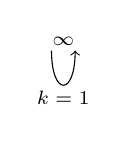
\begin{tikzpicture}[scale = 0.3,baseline]
            \node at (0.5,1.4) {\scriptsize$\infty$};
            \node at (0.5,-1) {\scriptsize$k=1$};
            \path[->] (0,1) edge [bend right = 90,looseness=5] (1,1);
        \end{tikzpicture} \ 
    \ker (F - \lambda I)^k = \ker (F - \lambda I)^N \]
\end{df} 
\begin{uw} $V_\lambda < V^\lambda$ \end{uw} 
\begin{ft} $V^\lambda$ jest $F-$ niezmiennicza \end{ft} 
\begin{dd} 
    $v \in V^\lambda = \ker (F - \lambda I)^N$ \\ 
    $(F - \lambda I)^N v = 0$
    $(F - \lambda I)^N (F(v)) = (F - \lambda I)^N ((F - \lambda I)v + \lambda v) = 
    \underscript{(F- \lambda I)^{N+1}v}{\verteq}{0} + \underscript{\lambda(F - \lambda I)v}{\verteq}{0}= 0$ \\ 
    czyli $F(v) \in \ker (F - \lambda I)^N$
\end{dd}
\begin{lem} 
    $V = \ker (F - \lambda I)^N \oplus \operatorname{Im} (F - \lambda I)^N$
    \begin{dd}  \hfill
        \begin{enumerate}[(1)] 
            \item $\dim\ker (F - \lambda)^N + \dim\operatorname{Im} ( F - \lambda I)^N = \dim V$
            \item $v \in \ker(F - \lambda I)^N \cap (\operatorname{Im}(F - \lambda I)^N)$ \\ 
                $v = (F - \lambda I)^N w$ \\ 
                $0 = (F - \lambda I)^N = (F - \lambda I)^{2N} w$, czyli $w \in \ker(F - \lambda I)^{2N} = 
                \ker (F - \lambda I)^N$, \\ 
                czyli $\ker () \cap \operatorname{Im}() = \{0\}$, czyli $v = 
                (F - \lambda Id)^N w = 0$
        \end{enumerate} 
    \end{dd} 
\end{lem} 
\begin{lem} 
    $\operatorname{Im}(F - \lambda I)^N$ jest $F - $ niezmiennicza. 
    \begin{dd} 
        $v = (F - \lambda I)^N w$ \\ 
        $F(v) = ((F - \lambda I) + \lambda I)(F - \lambda I)^N w = ((F - \lambda I)^{N+1} + \lambda(F - \lambda I)^N)w = 
        (F - \lambda I)^N ((F - \lambda I) + \lambda I)w = (F - \lambda I)(F(w)) \in \operatorname{Im}(F - \lambda I)^N$ \\ 
    (tzn. $(F - \lambda I)^N$ i $F$ komutują)
    \end{dd} 
\end{lem} 
\begin{wn} $V = V^{\lambda_1} \oplus \ldots \oplus V^{\lambda_k}$ \end{wn}
\begin{dd} 
    Indukcja względem k \\ 
    $1^{\circ} k=1 \\ \chi_F (x) = (\lambda_1 -x )^{\dim V}$ \\ 
    $B - $ baza $V ^{\lambda_1} < V$ \\ 
    $B'  - $ baza $\operatorname{Im} (F - \lambda_1 I)^N$ \\ 
    $C = B \cup B' - $ baza $V$ \\  
    $ m_C^C = \begin{pmatrix} 
        m_B^B(F|_{V^{\lambda_1}}) & 0 \\ 0 & m_{B'}^{B'} (F|_{\operatorname{Im}})
    \end{pmatrix}$ \\ 
    $\chi (F) = \chi(F|_{\lambda^k}) \chi(F|_{\operatorname{Im}})$ \\ 
    $\chi(F|_{\operatorname{Im}}) = (\lambda_1 - x)^s$ istnieje wektor własny dla $\lambda$ poza $V^\lambda$ 
    sprzeczność. Zatem $V^{\lambda_1} = V$ \\ 
    $2^{\circ} F: V \to V$ ma $k+1$ różnych wartości własnych. \\ 
    $ V = \underscript{\ker(F-\lambda I)^N}{\verteq}{V^{\lambda_1}} \oplus \operatorname{Im}(F - \lambda_1 I)^N$ \\ 
    $C = B \cup B'$ - baza $V$  \\ 
    $m_C^C (F) = \begin{pmatrix} m_B^B (F|_{V^\lambda})  &0 \\ 0 & m_{B'}^{B'} (F|_{\operatorname{Im}}) \end{pmatrix}$ \\ 
    $\chi(F) = \chi (F|_{V^{\lambda_1}}) \chi(F|_{\operatorname{Im}})$ \\ 
    z założenia indukcyjnego $V = V^{\lambda_1} \oplus \ldots \oplus V^{\lambda_{k+1}}$
\end{dd} 
\subsection{Pojedyńcza klatka Jordana} 
$V = V^\lambda$ \\ 
$F: V \to V$, tzn $\chi_F (x) = (\lambda-x)^{\dim V}$ \\
cel 2: 
$m_B^B (F) = \begin{pmatrix} \lambda & 1 & & & & \\ 
                                     & \lambda & & & & \\
                                     & & \ddots & & & \\ 
                                     & & & \lambda & 1 & \\ 
                                     & & & & \lambda & 1 \\
                                     & & & & & \lambda
                                    \end{pmatrix} $ \\ 
$m_B^B (F) = \begin{pmatrix} J_1 & & \\ & \ddots & \\ & & J_s \end{pmatrix}$, gdzie
$J_i = \begin{pmatrix} \lambda & 1 & & & \\ & \ddots & \ddots & & \\ 
        & & \ddots & 1 \\ & & &  \lambda \end{pmatrix}$ \\ 
$G \overset{\text{ozn.}}{=} F - \lambda I$ \\ 
$m_B^B (G) = \begin{pmatrix} J_1 ' & & \\ & \ddots & \\ & & J_s' \end{pmatrix}$, gdzie
$J_i' = \begin{pmatrix} 0 & 1 & & & \\ & \ddots & \ddots & & \\ 
            & & \ddots & 1 \\ & & &  0 \end{pmatrix}$ \\ 
$m_B^B (G) = \begin{pmatrix} 0 & 1 & & & & \\ 
                                     & 0 & & & & \\
                                     & & \ddots & & & \\ 
                                     & & & 0 & 1 & \\ 
                                     & & & & 0 & 1 \\
                                     & & & & & 0
                                    \end{pmatrix} $ \\
$\underline G \\ 
\begin{aligned} 
    b_3 \mapsto b_2 \mapsto b_1 \mapsto &0 \\ 
    b_5 \mapsto b_4 \mapsto &0 \\ 
    b_7 \mapsto b_6 \mapsto &0 
\end{aligned} $ \\ 
\underline{CEL}: Jeśli $G: V \to V$ ma własność $G^N = 0$ dla pewnego $N$ (tzn. $G$ jest nilpotentna), to 
    istnieje baza $V$ postaci $\begin{aligned} b_1, G(b_1),&\ldots,G^{k_1 -1} (b_1) \\ 
                                               b_2, G(b_2),&\ldots,G^{k_2 -1} (b_2) \\
                                                            &\vdots \\
                                               b_s, G(b_s),&\ldots,G^{k_s -1} (b_s) \end{aligned}$
    oraz $G^{k_i} (b_i) = 0$

\underline{Dowód przed indukcję względem $\dim V$} \\ 
Niech $W = \ker G < V$ \\ 
Jeśli $W = V$ to bierzemy dowolną bazę $V$: mamy 
$\begin{aligned} b_1 \mapsto &0 \\ \vdots \\ b_{\dim V} \mapsto &0 \end{aligned} $ \\ 
Jeśli $W \lneq V$, to stosujemy założenie indukcyjne do $\overline F: V/_W \to V/_W$ \\ 
zatem $V /_W$ ma bazę $\overline B = \{G^j (b_i) + W, i = 1,\ldots,s; j = 0,1,\ldots,k_i-1 \}$ \\ 
$G^j (b_i) \in V$ lnz, bo $ 0 = \sum \alpha_{ij} G^j (b_i)$, to $\sum \alpha_{ij}(G^j(b_i) + W) = 0+W$, czyli 
$\alpha_{ij} = 0$ \\ 
$B = \{ G^j (b_i) : i = 1,\ldots,s; j = ,1,\ldots,k_i \} \cup \underscript{\{c_1,\ldots,c_s\}}{\cap}{\ker G = W}$
$0 = \sum \alpha_{ij} G^j (b_i) = G( \sum \alpha_{ij} G^{j-1} (b_i))$, a to już wiemy, że jest lnz, czyli $\alpha_{ij} = 0$.

\section{Formy kwadratowe} 
$f: \mathbb R \to \mathbb R$, gładka \\ 
$f(x) \simeq f(x_0) + f'(x_0)(x-x_0) + \frac{f''(x_0)}{2}(x-x_0)^2$ \\ 
\begin{tikzpicture}
    \begin{axis}[xmin=-5,xmax=5,ymax=2,ymin=-2,samples=500]
        \addplot[domain=-5:5,black] (x,0.008*x^5 - 0.16*x^3 +x);
        \addplot[domain=-5:5,red] (x,0.73*x + 0.15);
    \end{axis}
\end{tikzpicture}
\begin{tikzpicture}
    \begin{axis}[xmin=-5,xmax=5,ymax=2,ymin=-2,samples=500]
        \addplot[domain=-5:5,black] (x,-0.16*x^3+x);
        \addplot[domain=-5:5,red] (x,0.98);
    \end{axis}
\end{tikzpicture} \\
$f: \mathbb R ^2 \to \mathbb R$ \\
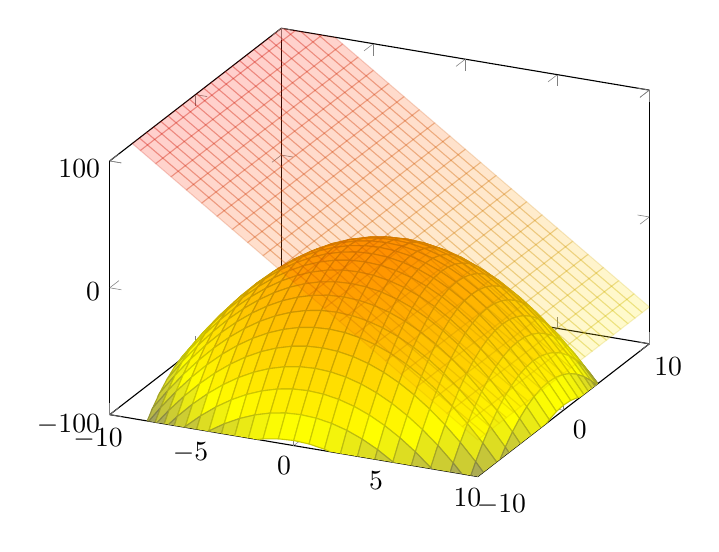
\begin{tikzpicture}
    \begin{axis}[xmin=-10,xmax=10,ymin=-10,ymax=10,zmin=-100,zmax=100]
    \addplot3[surf,domain=-10:10] {-x^2-y^2+4};
    \addplot3[surf,domain=-10:10,opacity=0.2] {-10*x+29};
  \end{axis}
\end{tikzpicture}\\
$f(\begin{pmatrix} x \\ y \end{pmatrix}) \simeq ax + by +c$ \\ 
$f(x,y) \simeq f(x_0,y_0) + f_x (x_0,y_0)(x-x_0) + f_y(x_0,y_0)(y-y_0)$
\begin{prz} 
    $f(x,y) = 2x^2 + 3xy + y^3 \\ 
    f_x = 4x + 3y \\ 
    f_y = 3x + 3x^2$
\end{prz}
$f(x,y) \simeq f(x_0,y_0)
\begin{aligned}[t]
    &+ f_x(x_0,y_0) (x-x_0) \\
    &+ f_y(x_0,y_0) (y-y_0) \\ 
    &+ d (x-x_0)^2  \\ 
    &+ e (y-y_0)^2  \\ 
    &+ f (x-x_0)(y-y_0)
\end{aligned} $ \\ 
$ f_{xx} = 4 \\ f_{xy} = 3 \\ f_{yx} = 3 \\ f_yy = 6y$ \\
$\begin{pmatrix} 
    f_{xx} & f_{xy} \\ f_{yx} & f{yy} 
\end{pmatrix}$ \\ 
$f: \mathbb R^n \to R$\\ 
$\begin{pmatrix} 
    f_{x_1 x_1} & f_{x_1 x_2} & \ldots \\ 
        & \ddots & \\ 
        & & 
\end{pmatrix}$ 
\begin{prz} 
    $a x^2 + b xy + cy^2 = \begin{pmatrix} x & y \end{pmatrix}
    \begin{pmatrix} a & \frac{b}{2} \\ \frac{b}{2} & c \end{pmatrix} 
    \begin{pmatrix} x \\ y \end{pmatrix}$
\end{prz} 
\begin{prz} 
    $a x^2 + by^2 + cz^2 + dxy + eyz + fxz = 
    \begin{pmatrix} x & y & z \end{pmatrix} 
    \begin{pmatrix} a & \frac{d}{2} & \frac{f}{2} \\ 
                    \frac{d}{2} & b & \frac{e}{2} \\ 
                \frac{f}{2} & \frac{e}{2} & c \end{pmatrix} 
    \begin{pmatrix} x \\ y \\ z \end{pmatrix} $
\end{prz} 
\begin{df} 
    Forma dwulinoiwa na przestrzeni liniowej $V$, to dwulinoiwa funkcja $\phi: V \times 
    V \to K$
\end{df}
\begin{ft} 
    Niech $B = (b_1,\ldots,b_n)$ będzie bazą $V$, a $\phi: V \times V \to K$ formą
    dwuliniową. Wówczas \[ \phi(v,w) = ([v]_B)^\top A [w]_B\] gdzie $A = (a_{ij}) 
    \in M_{n \times n} (K) \ a_{ij} = \phi(b_i,b_j)$. \\ 
    Macierz A oznaczamy $m^{BB}(\phi)$ i nazywamy macierzą formy dwuliniowej $\phi$ 
    w bazie $B$.
\end{ft} 
\begin{dd} $v_i,w_i \in K, b_i \in V$ \\ 
    $[v]_B = \begin{pmatrix} v_1 \\ \vdots \\ v_n \end{pmatrix},\ 
     [w]_B = \begin{pmatrix} w_1 \\ \vdots \\ w_n \end{pmatrix}$ \\ 
    $\phi(v,w) = \phi( \sum\limits_i v_i b_i, \sum\limits_j w_j b_j) = 
    \sum\limits_i \sum\limits_j v_i w_j \phi (b_i,b_j) = 
    \begin{pmatrix} v_1 &\dots& v_n \end{pmatrix}
    \begin{pmatrix} \phi(b_1,b_1) & \dots & \phi(b_1,b_n) \\ 
                    \vdots & \vdots & \vdots \\ 
                \phi(b_n,b_1) & \dots & \phi(b_n,b_n) \end{pmatrix}
    \begin{pmatrix} w_1 \\ \vdots \\ w_n \end{pmatrix}$
\end{dd}
\begin{ft} 
    $B = (b_1,\ldots,b_n) - $ baza przestrzeni liniowej $V$, zaś $A \in M_{n \times n}(K)$
    Wówczas \[ \phi(v,w) = ([v]_B)^\top A [w]_B\] jest formą dwuliniową.
\end{ft} 
\begin{dd} ~\\ 
    $\phi(\alpha_1 v_1 + \alpha_2 v_2,w) = ([\alpha_1 v_1+\alpha_2 v_2]_B)^\top 
    A[w]_B = (\alpha_1([v_1]_B)^\top + \alpha_2([v_2]_B)^\top)A [w]_B = 
    \alpha_1 \phi(v_1,w) + \alpha \phi(v_2,w)$ Analogicznie dla drugiej współrzędnej. 
\end{dd} 
\begin{ft} 
    $V - $ przestrzeń liniowa \\ 
    $B, C $ bazy $V$ \\ 
    $\phi: V \times V \to K$ forma dwulinowa 
    \[ m^{CC} (\phi) = (m_{\cancel{B}}^C(id))^\top m^{\cancel{B}\bcancel{B}}
    (\phi) (m_{\bcancel{B}}^C(id)) = P^T m^{BB}(\phi) P\]
\end{ft} 
\begin{dd} 
    $\phi (v,w) = ([v]_B)^\top m^{BB}(\phi) [w]_B = (m_B^C(id)[v]_C)^\top m^{BB}(\phi) 
    (m_B^C(id)[w]_C) = \\ ([v]_C)^\top 
    \underbrace{((m_B^C (id))^\top m^{BB}(\phi) m_B^C(id))}_{m^{CC}(\phi)} [w]_C$
\end{dd} 
\begin{df} 
    Dwuliniowa forma $\phi: V \times V \to K$ jest: \\ 
        symetryczna, jeśli $(\forall v,w \in V) \phi(v,w) = \phi(w,v)$ \\ 
        antysymetryczna, jeśli $(\forall v,w \in V) \phi(v,w) = - \phi(w,v)$
\end{df} 
\begin{ft} 
    Forma dwuliniowa $\phi$ jest (anty)symetryczna iff $m^{BB} (\phi)$ jest 
    (anty)symetryczna w pewnej (=dowolnej) bazie $B$. 
\end{ft} 
\begin{dd} ~\\ 
    $\phi(v,w) = ([v]_B)^\top A [w]_B$ \\ 
    $\phi(w,v) = (([w]_B)^\top A [v]_B)^\top = ([v]_B)^\top A^\top [w]_B$
\end{dd} 
\begin{df} 
    Funkcję $Q: V \to K$ nazywamy \underline{formą kwadratową} jeśli $Q(v) = \phi(v,v)$ 
    dla pewnej formy dwuliniowej $\phi$. (oznaczamy: $Q = \widetilde \phi$)
\end{df} 
\begin{prz} 
    $Q: \mathbb R^2 \to \mathbb R \ Q(\begin{pmatrix} x \\ y \end{pmatrix}) = ax^2 +bxy+ 
    cy^2 = \begin{pmatrix} x & y \end{pmatrix} \begin{pmatrix} a & \frac{b}{2} \\ 
    \frac{b}{2} & c \end{pmatrix} \begin{pmatrix} x \\ y \end{pmatrix}$
\end{prz} 
forma dwuliniowa $\phi \longrightarrow$ forma kwadratowa $Q(v) = \phi(v,v)$
\begin{uw} Jeśli $\phi,\phi'$ to formy dwuliniowe, $A = m^{BB}(\phi),\ A'=m^{BB}
(\phi)$ \\ 
$\forall i,j (a_{ij} + a_{ji} = a'_{ij} + a'_{ji})$, to $\widetilde\phi = \widetilde
{\phi}\, '$
\end{uw} 
\begin{uw} Od tej pory $\operatorname{char} K \neq 2$ \end{uw}
\begin{uw} $Q: V \to K$ forma kwadratowa \\ 
    $Q(v) = ([v]_B)^\top A [v]_B$, dla pewnej macierzy $A \in M_{n \times n}(K)$
    $B = (b_1,\ldots,b_n)$ - baza $V$. \\ 
    $a_{ii} = Q(b_i) = \phi(b_i,b_i)$
    $i \neq j \ a_{ij} = \phi(b_i,b_j)$ \\ 
    $Q(v+w) = \phi(v+w,v+w) = \phi(v,v)+\phi(v,w)+\phi(w,v)+\phi(w,w) = Q(v)
    + Q(w) + 2\phi(v,w)$
    czyli $a_{ij} = \frac{1}{2} (Q(b_i+b_j) - Q(b_i) - Q(b_j))$
\end{uw} 
\begin{ft}[wzór polaryzacyjny] 
    \[ \phi(v,w) = \frac{1}{2} (Q(v+w) - Q(v) - Q(w)) \]
    Dla dowolnej formy kwadratowej $Q = \widetilde \phi$ o ile $\phi$ symetryczne. 
\end{ft}
\begin{wn} 
    forma dwuliniowa symetryczna $\phi \longleftrightarrow$ forma kwadratowa $Q(v) = 
    \phi(v,v)$ \hfill (bijekcja)
\end{wn} 
\begin{uw} 
    Dla uproszczenia często używamy tego samego oznaczenia dla formy kwadratowej oraz 
    symetrycznej formy dwuliniowej od której ona pochodzi
\end{uw} 
\begin{ft} 
    Funkcja $Q: V \to K$ jest formą kwadratową iff spełnia obydwa warunki:
    \begin{enumerate}[(1)]
        \item $\phi(v,w) := \frac{1}{2} (Q(v+w) - Q(v) - Q(w))$ jest formą dwulinową. 
        \item $\forall t \in K \ \forall v \in V ( Q(tv) = t^2 Q(v))$
    \end{enumerate} 
\end{ft} 
\begin{dd} 
    \begin{itemize} \hfill
        \item[$\Downarrow$] \begin{enumerate}[(1)] 
                                \item wzór polaryzacyjny 
                                \item $Q(tv) = \phi(tv,tv,)=t^2 \phi(v,v) = t^2 Q(v)$
                            \end{enumerate} 
        \item[$\Uparrow$] $\phi(v,w) = \ldots $ forma dwuliniowa \\ 
            chcemy $Q = \widetilde \phi$ \\ 
            $Q(v) \overset{?}{=} \phi(v,v)$ \\ 
            $\phi(v,v) = \frac{1}{2} (Q(2v)-2Q(v)) \overset{2}{=}Q(v)$
    \end{itemize} 
\end{dd} 
\begin{tw}[o diagonalizacji formy kwadratowej] 
    $Q: V \to K$ forma kwadratowa \\ 
    Wówczas istnieje taka baza w przestrzeni $V$, że $m^{BB}(Q)$ jest diagonalna.\\
    (tzn. $Q(v) = \alpha_1 v_1^2 + \alpha_2 v_2^2 + \ldots + \alpha_n + v_n^2$ dla 
    $[v]_B = \begin{pmatrix} v_1 \\ \vdots \\ v_n \end{pmatrix}$)
\end{tw} 
\begin{dd} 
    $Q(x_1,\ldots,x_n) = \sum\limits_{i \le j} a_{ij} x_i x_j$ \\ 
    \underline{\textbf{Metoda Lagrange'a}} 
    \begin{enumerate}[(1)]
        \item Jesli $a_{ii} \neq 0$, dla pewnego $i$ b.s.o $i = 1$ \\ 
            $a_{11}x_1^2 + a_{12}x_1x_2 + \ldots a_{1n}x_1x_n + \sum\limits_{2 \le i \le j
                \le n} a_{ij}x_ix_j = a_{11}\underscript{(x_1 + \frac{a_{12}}{2a_{11}}x_2 + 
            \ldots + \frac{a_{1n}}{2a_{11}} x_n)^2}{\verteq\text{def}}{x'1} +
            \sum\limits_{2 \le i \le j \le n} a_{ij} x_i x_j = a_{11} (x'_1)^2 + 
            \sum\limits_{2 \le i \le j \le n} $ Dalej indukcyjnie. 
        \item Jeśli $a_{ii} = 0$ dla każdego $i$ to znajdujemy $a_{ij} \neq 0$ i 
            przeprowadzamy zamianę zmiennych $a_{ij}x_i x_j = 
            \frac{a_{ij}}{4} (\underscript{x_i + x_j}{\verteq}{x'_i})^2 - 
            \frac{a_{ij}}{4}(\underscript{x_i - x_j}{\verteq}{x'_j})^2 $
    \end{enumerate}
\end{dd}
od tej pory $K = \mathbb R$
\begin{df} 
    Formę kwadrotową $Q: V \to \mathbb R$ nazywamy: 
    \begin{itemize} 
        \item dodatnio określona jeśli $Q(v) > 0$ dla każdego $v \neq 0$ 
        \item ujemne określona, jesli $Q(v) < 0$ dla każdego $v \neq 0$ 
        \item dodatnio półokreślona $Q(v) \ge 0$ dla każdego $v \neq 0$ 
        \item ujemnie półokreślona $Q(v) \le 0$ dla każdego $v \neq 0$ 
    \end{itemize} 
\end{df} 
\begin{tw}[tw. Sylvestera] ~\\
    $Q: V \to \mathbb R$ forma kwadratowa \\ 
    $B -$ baza $V$ \\ 
    $m^{BB}(Q) = (a_{ij})_{1 \le i, j \le n}$ \\ 
    Wtedy $Q$ jest dodatnio określona $\Leftrightarrow$ $\det(a_{ij})_{1 \le i,j \le k}
    > 0$ dla $k = 1, 2, \ldots, n$
\end{tw} 
\begin{figure} 
    \centering
    \begin{tikzpicture}
        \draw (0,0) -- (5,0);
        \draw (0,0) -- (0,-5);
        \draw (1,0) -- (1,-1); 
        \draw (0,-1) -- (1,-1); 
        \draw (2,0) -- (2,-2); 
        \draw (0,-2) -- (2,-2);
        \draw (3,0) -- (3,-3); 
        \draw (0,-3) -- (3,-3); 
        \draw (5,0) -- (5,-5); 
        \draw (0,-5) -- (5,-5); 
        \draw [fill] (3.5,-3.5) circle[radius=0.025];
        \draw [fill] (4,-4) circle[radius=0.025];
        \draw [fill] (4.5,-4.5) circle[radius=0.025];
    \end{tikzpicture}
\caption{Ogólna idea tw Sylvestera, kolejne kwadraty oznaczają kolejne $(a_ij)_{1 \le i,j \le k} $ dla kolejnych $k$}
\end{figure} 
\begin{dd} \hfill
    \begin{itemize} 
        \item[$\Rightarrow$]$W = \operatorname{Lin} \{b_1,\ldots,b_k\} < V$ \\ 
                            $Q|_W: W \to \mathbb R$ dodatnio określona forma kwadratowa\\
                            Istnieje baza $C^{(k)}$, w której $Q|_W$ diagonalizowalna. \\
                            $B^{(k)}=(b_1,\ldots,b_n)$ \\ 
                            $m^{B^{(k)}B^{(k)}}(Q|_W)=(a_{ij})_{1 \le i,j\le k}=A^{(k)}$
                            $A^{(k)} = P^\top 
                            \begin{pmatrix} \lambda_1 & & \\ & \ddots & \\ & & \lambda_k
                            \end{pmatrix} P$ \\ 
                            $\lambda_1, \ldots,\lambda_k > 0$ \\ 
                            $\lambda_1 x_1^2 + \ldots + \lambda_k x_k^2 > 0$  
                            $\det(A^{(k)}) = \det P^\top \det P \lambda_1\dots\lambda_k=
                            (\det P)^2 \lambda_1 \dots \lambda_k > 0$
        \item[$\Leftarrow$]$\begin{aligned}[t] 
                            b'_k &= b_k - \sum\limits_{i =1}^{k-1} \frac{Q(b_k,bi')}{Q(
                            b_i',b_i')} b_i'\\ 
                            \vdots \\
                            b'_2 &= b_2 - \frac{Q(b_2,b_1')}{Q(b_1',b_1')} b'_1 \\
                            b'_1 &= b_1
                            \end{aligned}$ \\ 
                            Dowód indukcyjny następującego pakietu warunków: 
                            \begin{enumerate}
                                \item $\operatorname{Lin}\{b_1,\ldots,b_s\} = 
                                       \operatorname{Lin}\{b'_1,\ldots,b'_s\}$ 
                                \item $Q(b_s',b_s') > 0$ 
                                \item $Q(b_i',b_j') = 0$ dla $i \neq j,\ i j \le s$
                            \end{enumerate} 
                            $1^\circ$ oczywiste \\ 
                            $2^\circ$ 
                            \begin{itemize} 
                                \item[$(1)$]$\operatorname{Lin}\{b_1',\ldots,b_{s+1}'\}\ni
                                    \underbracket{b_1,\ldots,b_s}_{\text{zał indukcyjne}}
                                    b_{s+1} \leftarrow$ z defnicji $b_{s+1}$, czyli \\ 
                                    $\operatorname{Lin}\{b_1,\ldots,b_{s+1}\}= 
                                    \operatorname{Lin}\{b'_1,\ldots,b'_{s+1}\}$ 
                                \item[$(3)$] Dla $j \le s \ Q(b_j',b_{s+1}') = 
                                    Q(b_j',b_{s+1}) - \sum\limits_{i=1}^s
                                    \frac{Q(b_{s+1},b_i')}{Q(b_i',b_i')}b_i'=Q(b_j',b_{s+1
                                    })-\sum\limits_{i=1}^s \frac{Q(b_{s+1},b_i')}{Q(b_i',
                                    b_i')}Q(b_j',b_i')=Q(b_j',b_{s+1})-\frac{Q(b_{s+1},
                                    b_j')}{\cancel{Q(b_j',b_j')}} \cancel{Q(b_j',b_j')}=0$
                                \item[$(2)$] $m^{BB} (Q|_{\operatorname{Lin}\{b_1,\ldots,
                                    b_{s+1}\}})=A^{s+1} \\ 
                                    m^{B'B'}(Q|_{\operatorname{Lin}\{b'_1,\ldots,
                                    b'_{s+1}\}})=\begin{pmatrix} \lambda_1 & & 0 \\ 
                                    & \ddots & \\ 0 & & \lambda_{s+1}\end{pmatrix} 
                                    $ Ale wiemy $det A^{(s)} > 0$ \\ 
                                        $A^{(s+1)} = P^\top \begin{pmatrix} \lambda_1 & &
                                            \\ & \ddots & \\& &\lambda_{s+1}\end{pmatrix}
                                    \\ 0 < \det A^{(s)} = (\det P)^2 \lambda_1 \ldots 
                                    \lambda_s \lambda_{s+1}$ \\ czyli $\lambda_{s+1} > 0$
                                    \\ Zatem dla $B' = \{b_1',\ldots,b_n'\}$, to 
                                    $m^{B'B'}(Q) = \begin{pmatrix} \lambda_1 & & 
                                    \\ & \ddots & \\ & & \lambda_n \end{pmatrix}
                                    \lambda_1,\ldots,\lambda_n > 0$, czyli $Q$ dodatnie
                                    określone. 
                            \end{itemize} 
    \end{itemize} 
\end{dd} 
